\documentclass[
	12pt,
    a4paper,
    egregdoesnotlikesansseriftitles, % Überschriften haben gleichen Font wie restlicher Text
    toc=chapterentrywithdots,
    oneside, openany,
    % twoside,openright,
    titlepage,
    parskip=half,
    headings=normal,  % reduces heading size
    listof=totoc,
    bibliography=totocnumbered,
    index=totoc,
    captions=tableheading,  % caption below table
    % chapterprefix,
    listof=flat,
    numbers=noenddot, % kein Punkt nach Nummerierung im Inhaltsverzeichnis
    final]
    {scrbook}
    
% details about your thesis
\newcommand{\titel}{Discrimination in Algorithms (Face Recognition)}
\newcommand{\artderarbeit}{Studienarbeit}  % {Bachelorarbeit,Masterarbeit}
\newcommand{\autor}{Ronny Pollak}
\newcommand{\modul}{Intercultural Communications} 
%\newcommand{\modulzusatz}{Strategien,\,Architekturen\,und\,Algorithmen}
\newcommand{\matrikelnr}{3694422}
\newcommand{\dozent}{Wolfgang Jockusch}
\newcommand{\abgabedatum}{27.01.2023}
\newcommand{\keywords}{key, words}
%\newcommand{\studentname}{key, words}
%\newcommand{\studentMatnr}{key, words}
\newcommand{\studentStudiengang}{Master Informatik}


% custom head and foot
\usepackage[automark]{scrlayer-scrpage}
\pagestyle{scrheadings}
\ihead{\headmark}
\chead{}
\ohead{\pagemark}
\renewcommand*\chaptermarkformat{\chapappifchapterprefix{\ }% 
  \thechapter.\enskip}
% anderenfalls zu viel Abstand von Titeln zu oberem Seitenrand
\RedeclareSectionCommand[afterindent=false,beforeskip=0pt]{chapter}

\RedeclareSectionCommand[tocindent=0pt]{section}
\RedeclareSectionCommand[tocindent=0pt]{subsection}
%\RedeclareSectionCommand[tocnumwidth=70pt]{chapter}

\usepackage{scrhack}

% other packages
\usepackage[utf8]{inputenc}
\usepackage[T1]{fontenc}
\usepackage{lmodern,relsize,textcomp,csquotes}
\usepackage{amsmath,amsfonts}
\usepackage[ngerman,english]{babel}  % flip for German thesis
\usepackage[final]{graphicx}
\usepackage{setspace,geometry,xcolor}
\usepackage{makeidx}
\usepackage{paralist,ifthen,todonotes}
\usepackage{url}
\usepackage[toc]{glossaries}
\usepackage{pdfpages}

% table setup
\usepackage{longtable}
\usepackage{array}
\usepackage{ragged2e}
\usepackage{lscape}


\usepackage{hyperref}


% configure your listings style
\usepackage{listings}
\lstset{
	tabsize=3,
	extendedchars=true,
	frame=single,
	showstringspaces=true,
	numbers=left,
	numberstyle=\small,
	breakautoindent=true
}

% page setup
% \setlength{\topskip}{\ht\strutbox}
\geometry{paper=a4paper,left=2.5cm,top=3.0cm,bindingoffset=.8cm}
\onehalfspacing
%\frenchspacing
%\linespread{1.25} % NEU
\clubpenalty = 10000
\widowpenalty = 10000 
\displaywidowpenalty = 10000

% some commands
\newcommand{\ua}{\mbox{u.\,a.\ }}
\newcommand{\zB}{\mbox{z.\,B.\ }}
\newcommand{\dahe}{\mbox{d.\,h.,\ }}
\newcommand{\bzw}{\mbox{bzw.\ }}
\newcommand{\bzgl}{\mbox{bzgl.\ }}
\newcommand{\eg}{\mbox{e.\,g.\ }}
\newcommand{\ie}{\mbox{i.\,e.\ }}
\newcommand{\wrt}{\mbox{w.\,r.\,t.\ }}
\newcommand{\etal}{\mbox{\emph{et.\,al.\ }}}


% TODO remove if not needed...
\usepackage{blindtext}
\usepackage{todonotes}

% NEU musste für Bilder eingefügt werden
\usepackage{graphicx}
% NEU:damit Bilder nicht rumfloaten und an einer BESTIMMTEN Stelle sind -> [H]
\usepackage{float}

% Biblatex
\usepackage[backend=bibtex,style=alphabetic]{biblatex}
\addbibresource{refs.bib}


%\counterwithout{figure}{chapter}
% um nicht die Nummer des Kapitels bei der Figure Nummerierung zu stehen haben

\sloppy
%damit \textt nicht über die zeile hinaus geht

\begin{document}
\setcounter{secnumdepth}{3}  % numerate subsections
\setcounter{tocdepth}{2}  % ...but don't include them in toc


\frontmatter
\thispagestyle{empty}
\pdfbookmark[1]{Cover}{cov}
\begin{titlepage}

\begin{center}


\includegraphics[width=\linewidth]{figures/TH-Nuernberg-RGB.png}\\[1cm]
\LARGE{Fakultät Informatik}\\[2cm]

\huge
\textbf{\titel}\\[1cm]
%
\Large
\modul\\%[1cm]
\small


\vfill
\normalsize
%\newcolumntype{x}[1]{>{\raggedleft\arraybackslash\hspace{0pt}}p{#1}}
\begin{tabular}{rl}%{6cm}p{7.5cm}}
    \rule{0mm}{1ex}\textbf{Vorgelegt von:} & \autor \\
	\rule{0mm}{1ex}\textbf{Matrikelnummer:} & \hspace*{-0.5em}\begin{tabular}[t]{r}\matrikelnr\end{tabular} \\ 
	\rule{0mm}{1ex}\textbf{Studiengang:} & \studentStudiengang \\
	\rule{0mm}{1ex}\textbf{Dozent:} & \dozent \\ 
	\rule{0mm}{1ex}\textbf{Abgabedatum:} & \abgabedatum \\ 
\end{tabular} 		


\end{center}


%\vspace{-0.5cm}
%\singlespacing
%\small
%\noindent Dieses Werk einschließlich seiner Teile ist \textbf{urheberrechtlich geschützt}.
%Jede Verwertung außerhalb der engen Grenzen des Urheberrechtgesetzes ist ohne Zustimmung des Autors unzulässig und strafbar.
%Das gilt insbesondere für Vervielfältigungen, Übersetzungen, Mikroverfilmungen sowie die Einspeicherung und Verarbeitung in elektronischen Systemen.

\end{titlepage}

\tableofcontents

\listoffigures
\clearpage %\cleardoublepage % https://golatex.de/wiki/%5Ccleardoublepage

%\listoftables
%\clearpage %\cleardoublepage

\renewcommand{\lstlistlistingname}{List of Listings}  % change for German thesis
%\lstlistoflistings
\clearpage %\cleardoublepage

\mainmatter

\chapter{Introduction}
Discrimination in algorithms is a growing concern in the field of artificial intelligence (AI) and machine learning. 
Discrimination can occur in a number of ways, including bias in the training data or the algorithm itself. 
One specific area where discrimination has been identified is in facial recognition technology. This technology uses algorithms to analyze images of faces and match them to a database of known individuals.
This essay will discuss the ways in which discrimination can occur in algorithms, as well as providing specific examples of discrimination in facial recognition technology.

\chapter{Training and test data}
To understand how algorithms can discriminate a group of people you first have to understand how these algorithms work. 
When building an AI algorithm it has to be trained on a big amount of data. 
This is called the training data. 
In AI, training data is a set of data used to train an algorithmic model. 
In Figure \ref{fig:training} we can see a simplified illustration of a neural network as blackbox that is being trained on the training data.
The model uses this data to learn patterns and relationships in the data, which it can then use to make predictions or decisions on new, unseen data. 

\vspace{1em}
\begin{minipage}{\linewidth}
	\centering
	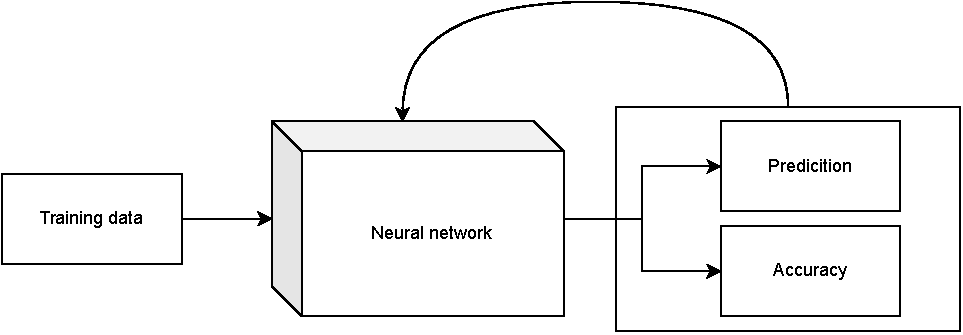
\includegraphics[width=0.8\textwidth]{figures/training.pdf}
	\captionof{figure}[Neural network as blockbox with training data]{Neural network as blockbox with training data}
	\label{fig:training}
\end{minipage}

On the other hand, is the test data. 
In Figure \ref{fig:training} we can see a simplified illustration of a neural network as blackbox that uses the test data to make predictions or decisions and compare them to the true values in the test data to evaluate its accuracy and reliability. 
In general, the training data is used to optimize the model and the test data is used to evaluate the model. \cite[p. 32-33]{khan_guide_2018}
%vll. rausmachen
%The data used in the training and test set can be biased in certain directions without the researchers knowing. It could have a higher proportion of males or of a single ethnicity. For example, if a face recognition system is being trained on a data set that mostly consists of white men it will have an easier time identifying white men which will result in a higher success rate.



\vspace{1em}
\begin{minipage}{\linewidth}
	\centering
	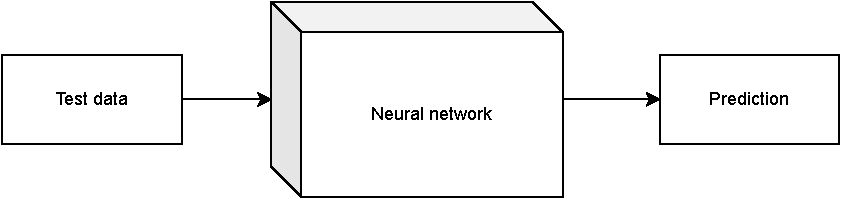
\includegraphics[width=0.8\textwidth]{figures/test.pdf}
	\captionof{figure}[Neural network as blockbox with test data]{Neural network as blockbox with test data}
	\label{fig:test}
\end{minipage}



\chapter{Issues with data}
%TODO Quelle und umschreiben!!
AI bias is an anomaly in the output of machine learning algorithms, due to the prejudiced assumptions made during the algorithm development process or prejudices in the training data.
 
There are many problems concerning the data that can make algorithms unreliable and lead to bias.
%One of them is poorly selected data.
%The designers of the algorithmic system may decide that certain data is important for the outcome of the algorithm and other data isn't.
%This can lead to disadvantages for a certain group of people. \cite[p. 7]{usa}
One of them is poorly selected data. As \textcite[p. 7]{usa} describe it, poorly selected data is “where the designers of the algorithmic system decide that certain data are important to the decision but not others. (...) Such issues can be regarded as qualitative errors, where human choices in the selection of certain datasets as algorithmic inputs over others are ill-advised (...) resulting in potentially discriminatory effects.”


Another problem is the selection bias.
Selection bias occurs when the set of data inputs to a model is not representative of a population, which can lead to conclusions that favor certain groups over others. \cite[p. 8]{usa}
For example, the training data for facial recognition AI algorithms is often composed of a higher number of faces from white people than from other races. This leads to difficulty in recognizing the faces of people from other races.
In a study by \textcite{buolamwini_gender_2018} the authors use the Fitzpatrick Skin Type classification system to characterize the gender and skin type distribution of two facial analysis benchmarks, IJB-A and Adience. 
They find that these datasets are overwhelmingly composed of lighter-skinned subjects, and introduce a new facial analysis dataset that is balanced by gender and skin type. 
They evaluate three commercial gender classification systems using their dataset and show that darker-skinned females are the most misclassified group, with error rates of up to 34.7\%. 
The maximum error rate for lighter-skinned males is 0.8\%. 
\cite[p. 1]{buolamwini_gender_2018}


People of color are disproportionately represented in the databases used by law enforcement for suspect identification, leading to a higher frequency of matches and a disproportionate number of true and false acceptances. \cite[p. 323-324]{bacchini_race_2019}
This can result in further discrimination when innocent individuals are stopped, searched, or arrested. 
These algorithms perpetuate the hidden, historical and systemic biases present in society that are transferred through their training data. \cite[p. 8]{usa}



\chapter{Solution approaches}
To prevent discrimination in algorithms, there are a number of steps that can be taken. 
One step is to ensure that the training data used to train algorithms is representative of the population it will be used on. 
This can be achieved by using diverse and inclusive data sets, or by using techniques such as data augmentation to make the training data more representative.
Data augmentation is a technique used to increase the amount of training data by adding modified copies of existing data or newly created synthetic data.
The aim of this technique is to reduce overfitting and promote better generalization when training machine learning models. \cite[p. 2]{nanni2022feature}
In the following Figure \ref{fig:augmentation} an example of a image data augmentation on an existing image of a person can be seen. 
This image gets modified in different ways to add more data.

\vspace{1em}
\begin{minipage}{\linewidth}
	\centering
	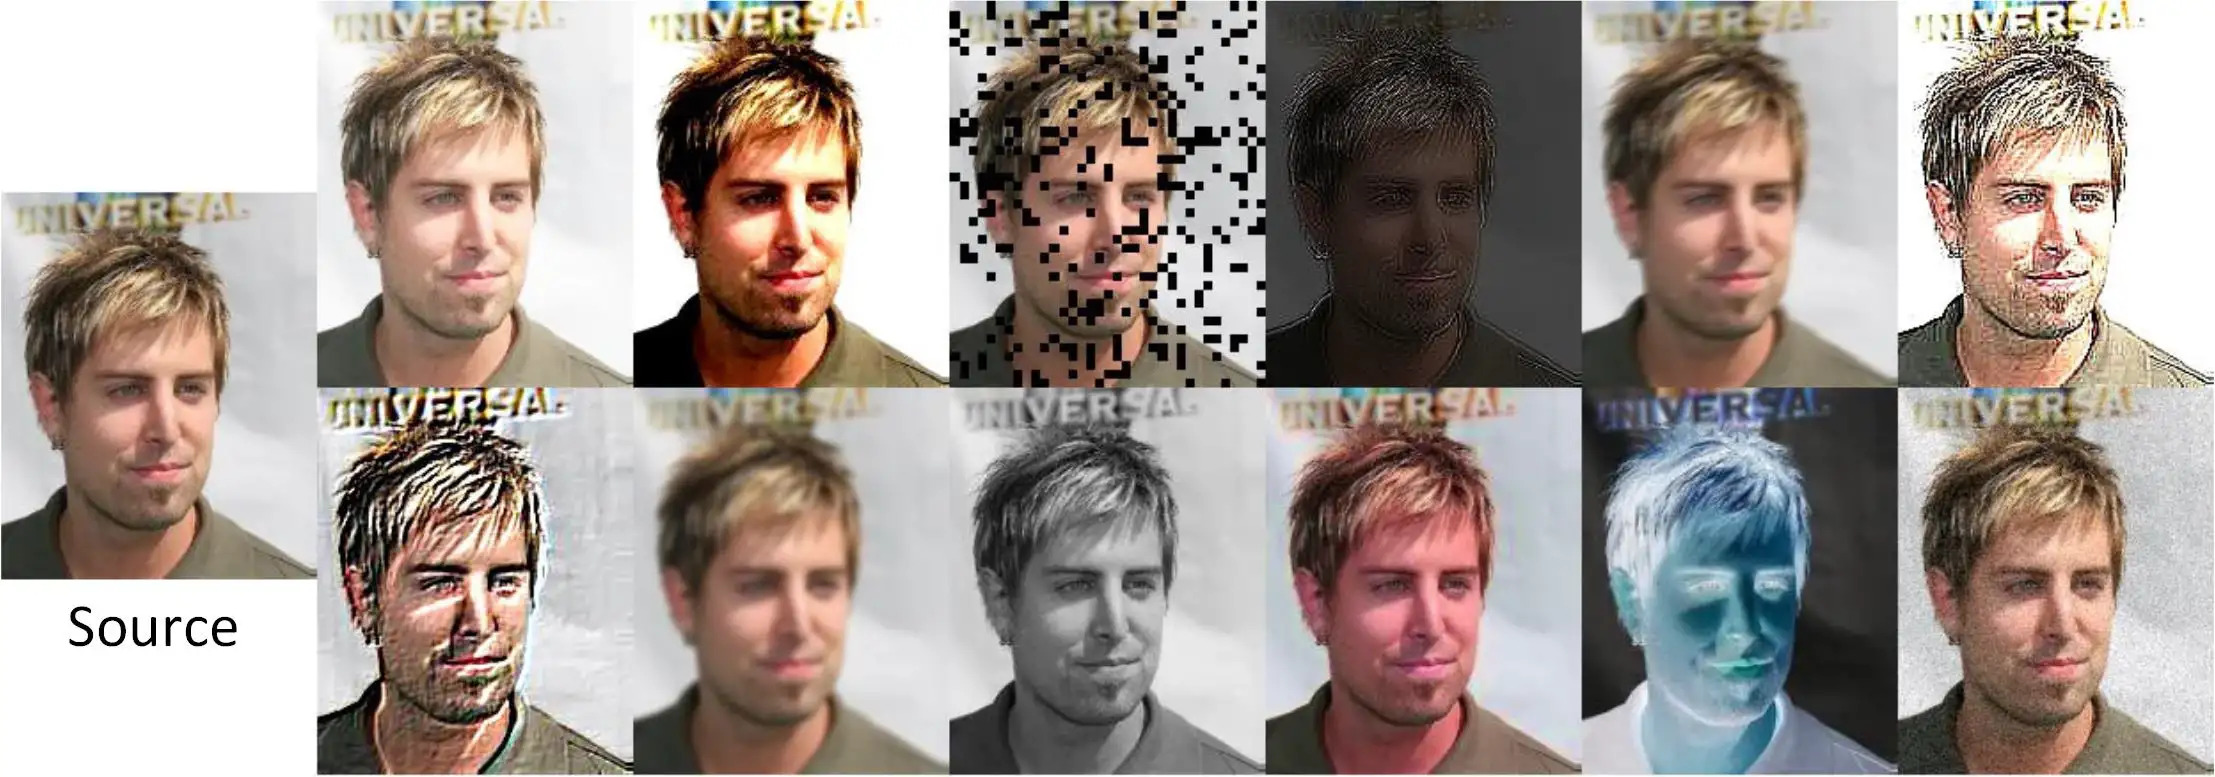
\includegraphics[width=0.8\textwidth]{figures/augmentation2.jpg}
	\captionof{figure}[Example data augmentation]{Example data augmentation \cite{singh_face_2020}}
	\label{fig:augmentation}
\end{minipage}

%Another step is to use techniques such as fairness or bias correction to reduce discrimination in the algorithm itself. 
%Fairness correction techniques can be used to ensure that an algorithm does not make incorrect assumptions or predictions about certain groups of people. 
%Bias correction techniques can be used to remove bias from the algorithm, such as by removing certain features or variables that are known to be associated with discrimination. [TODO Research und Quellen]


In the case of facial recognition technology, researchers and engineers can use techniques such as cross-dataset evaluation to test the accuracy of facial recognition algorithms on a diverse range of individuals. 
Cross-dataset evaluation is a method used to evaluate the performance of machine learning models on data that is different from the data that was used to train the model.
This is important because a model that performs well on the training data may not perform well on new, unseen data.
Cross-dataset evaluation helps to identify how well a model is likely to generalize to new data, and can be used to identify potential issues such as overfitting or bias in the training data.
This can help to identify and address any issues of bias or discrimination in the algorithm. \cite[p. 1-2]{yang_cross-datasets_2022} \cite[p. 3679-3680]{chen_cdevalsumm_2020}

%Pessach and Shmueli 
\textcite[p. 8-.10]{fairness} state that generally there are three fairness-enhancing mechanisms in machine learning: 
%\cite[p. 8-.10]{fairness}
\begin{itemize}
 \item \textbf{Pre-process} mechanisms involve changing the training data before it is fed into an machine learning algorithm, such as changing labels, reweighing instances, or modifying feature representations to make the classification fairer.
 \item \textbf{In-process} mechanisms involve modifying the machine learning algorithm during the training time, such as adding regularization terms, constraints, or adjusting decision tree split criteria to account for fairness.
 \item \textbf{Post-process} mechanisms are techniques used to adjust the predictions or threshold for classification made by a machine learning model after it has been trained, in order to reduce bias in the model's predictions. These techniques involve modifying the output of the model in some way, rather than changing the model itself.
\end{itemize}

%Specifically, post-process mechanisms can involve adjusting the predicted probabilities of different classes to balance the errors across different groups. For example, if a model is found to be more likely to predict the negative class for a certain group, the predicted probabilities for that group can be adjusted to reduce the bias. This approach is called re-weighting predictions.
%
%Another example of post-process mechanism is calibration, where the threshold for classification is adjusted to balance the true positive rate and the false positive rate across different groups. This can be done by adjusting the threshold of the decision function so that the model is more sensitive to certain groups in order to balance the false positive rate and false negative rate across different groups.

%Another approach is post-processing bias correction, which is based on the idea of using adversarial examples to correct bias in predictions. Adversarial examples are specifically crafted examples that are designed to fool a model into making incorrect predictions, and they can be used to identify and correct bias in the model's predictions.

%Adversarial Debiasing is another approach which utilizes an adversary network that tries to predict sensitive attributes from the representations learned by the main model. The adversary is trained simultaneously with the main model and the representations that are harder for the adversary to predict are considered less biased.
%
%It's important to note that post-process mechanisms are not a replacement for addressing bias in the model's training process, but rather a way to further improve the model's fairness after training. It's also important to keep in mind that post-processing may affect accuracy and could lead to other trade-offs, so it's important to evaluate the trade-offs before applying these techniques.

%Another important step in preventing discrimination in algorithms is to promote diversity and inclusivity in the field of AI and machine learning. 
%This includes encouraging more underrepresented groups such as women, people of colour, and people with disabilities to enter the field, and providing them with the resources and support they need to succeed. 
%It also includes creating a culture of inclusivity within the field, where all voices are heard and respected.
%
%
%Another step that can be taken to prevent discrimination in algorithms is to conduct regular audits and evaluations of the algorithms. 
%This can help to identify any issues of bias or discrimination and ensure that the algorithms are performing as intended. 
%Regular audits and evaluations can also be used to track the progress of the algorithm over time and to identify any areas where improvements can be made.

Promoting diversity and inclusivity in the field of AI and machine learning is crucial in preventing discrimination in algorithms. 
This includes actively seeking out and encouraging individuals from underrepresented groups such as women, people of color, and people with disabilities to enter the field, and providing them with the necessary resources and support to succeed. 
This can be achieved through initiatives such as mentorship programs, targeted recruitment efforts, and providing access to education and training opportunities. 
Creating a culture of inclusivity within the field is important, by fostering an environment where all voices are heard, respected, and valued, and actively working to address and eliminate discrimination and bias within the field.

Regular audits and evaluations of algorithms are also critical in preventing discrimination. These audits and evaluations can help to identify any issues of bias or discrimination in the algorithms, and ensure that they are performing as intended. 
The evaluations can also be used to track the progress of the algorithm over time and identify areas for improvement. 
Additionally, regular audits and evaluations can help to build trust and transparency with stakeholders, including customers, regulators, and the general public.



\chapter{Conclusion}
In conclusion, discrimination in algorithms is a growing concern in the field of AI and machine learning. 
Discrimination can occur in a number of ways, including bias in the training data or the algorithm itself. 
Facial recognition technology is one specific area where discrimination has been identified, as studies have found that facial recognition algorithms are less accurate when analyzing images of people with darker skin tones. 
Preventing discrimination in algorithms is a complex problem that requires a multifaceted approach. 
It is important to use diverse and inclusive data sets, and techniques such as fairness enhancing mechanisms, cross-dataset evaluation, and transparent algorithms. 
It is also crucial for policymakers to be aware of the issues of discrimination in algorithms and work to prevent discrimination in algorithms. 
Additionally, it is important to promote diversity and inclusivity in the field of AI and machine learning, to promote accountability and transparency, to use human feedback, and to engage with communities and stakeholders. 
By taking these steps, we can work towards ensuring that algorithms are fair, equitable, and do not perpetuate discrimination.


%\vspace{1em}
%\begin{minipage}{\linewidth}
%	\centering
%	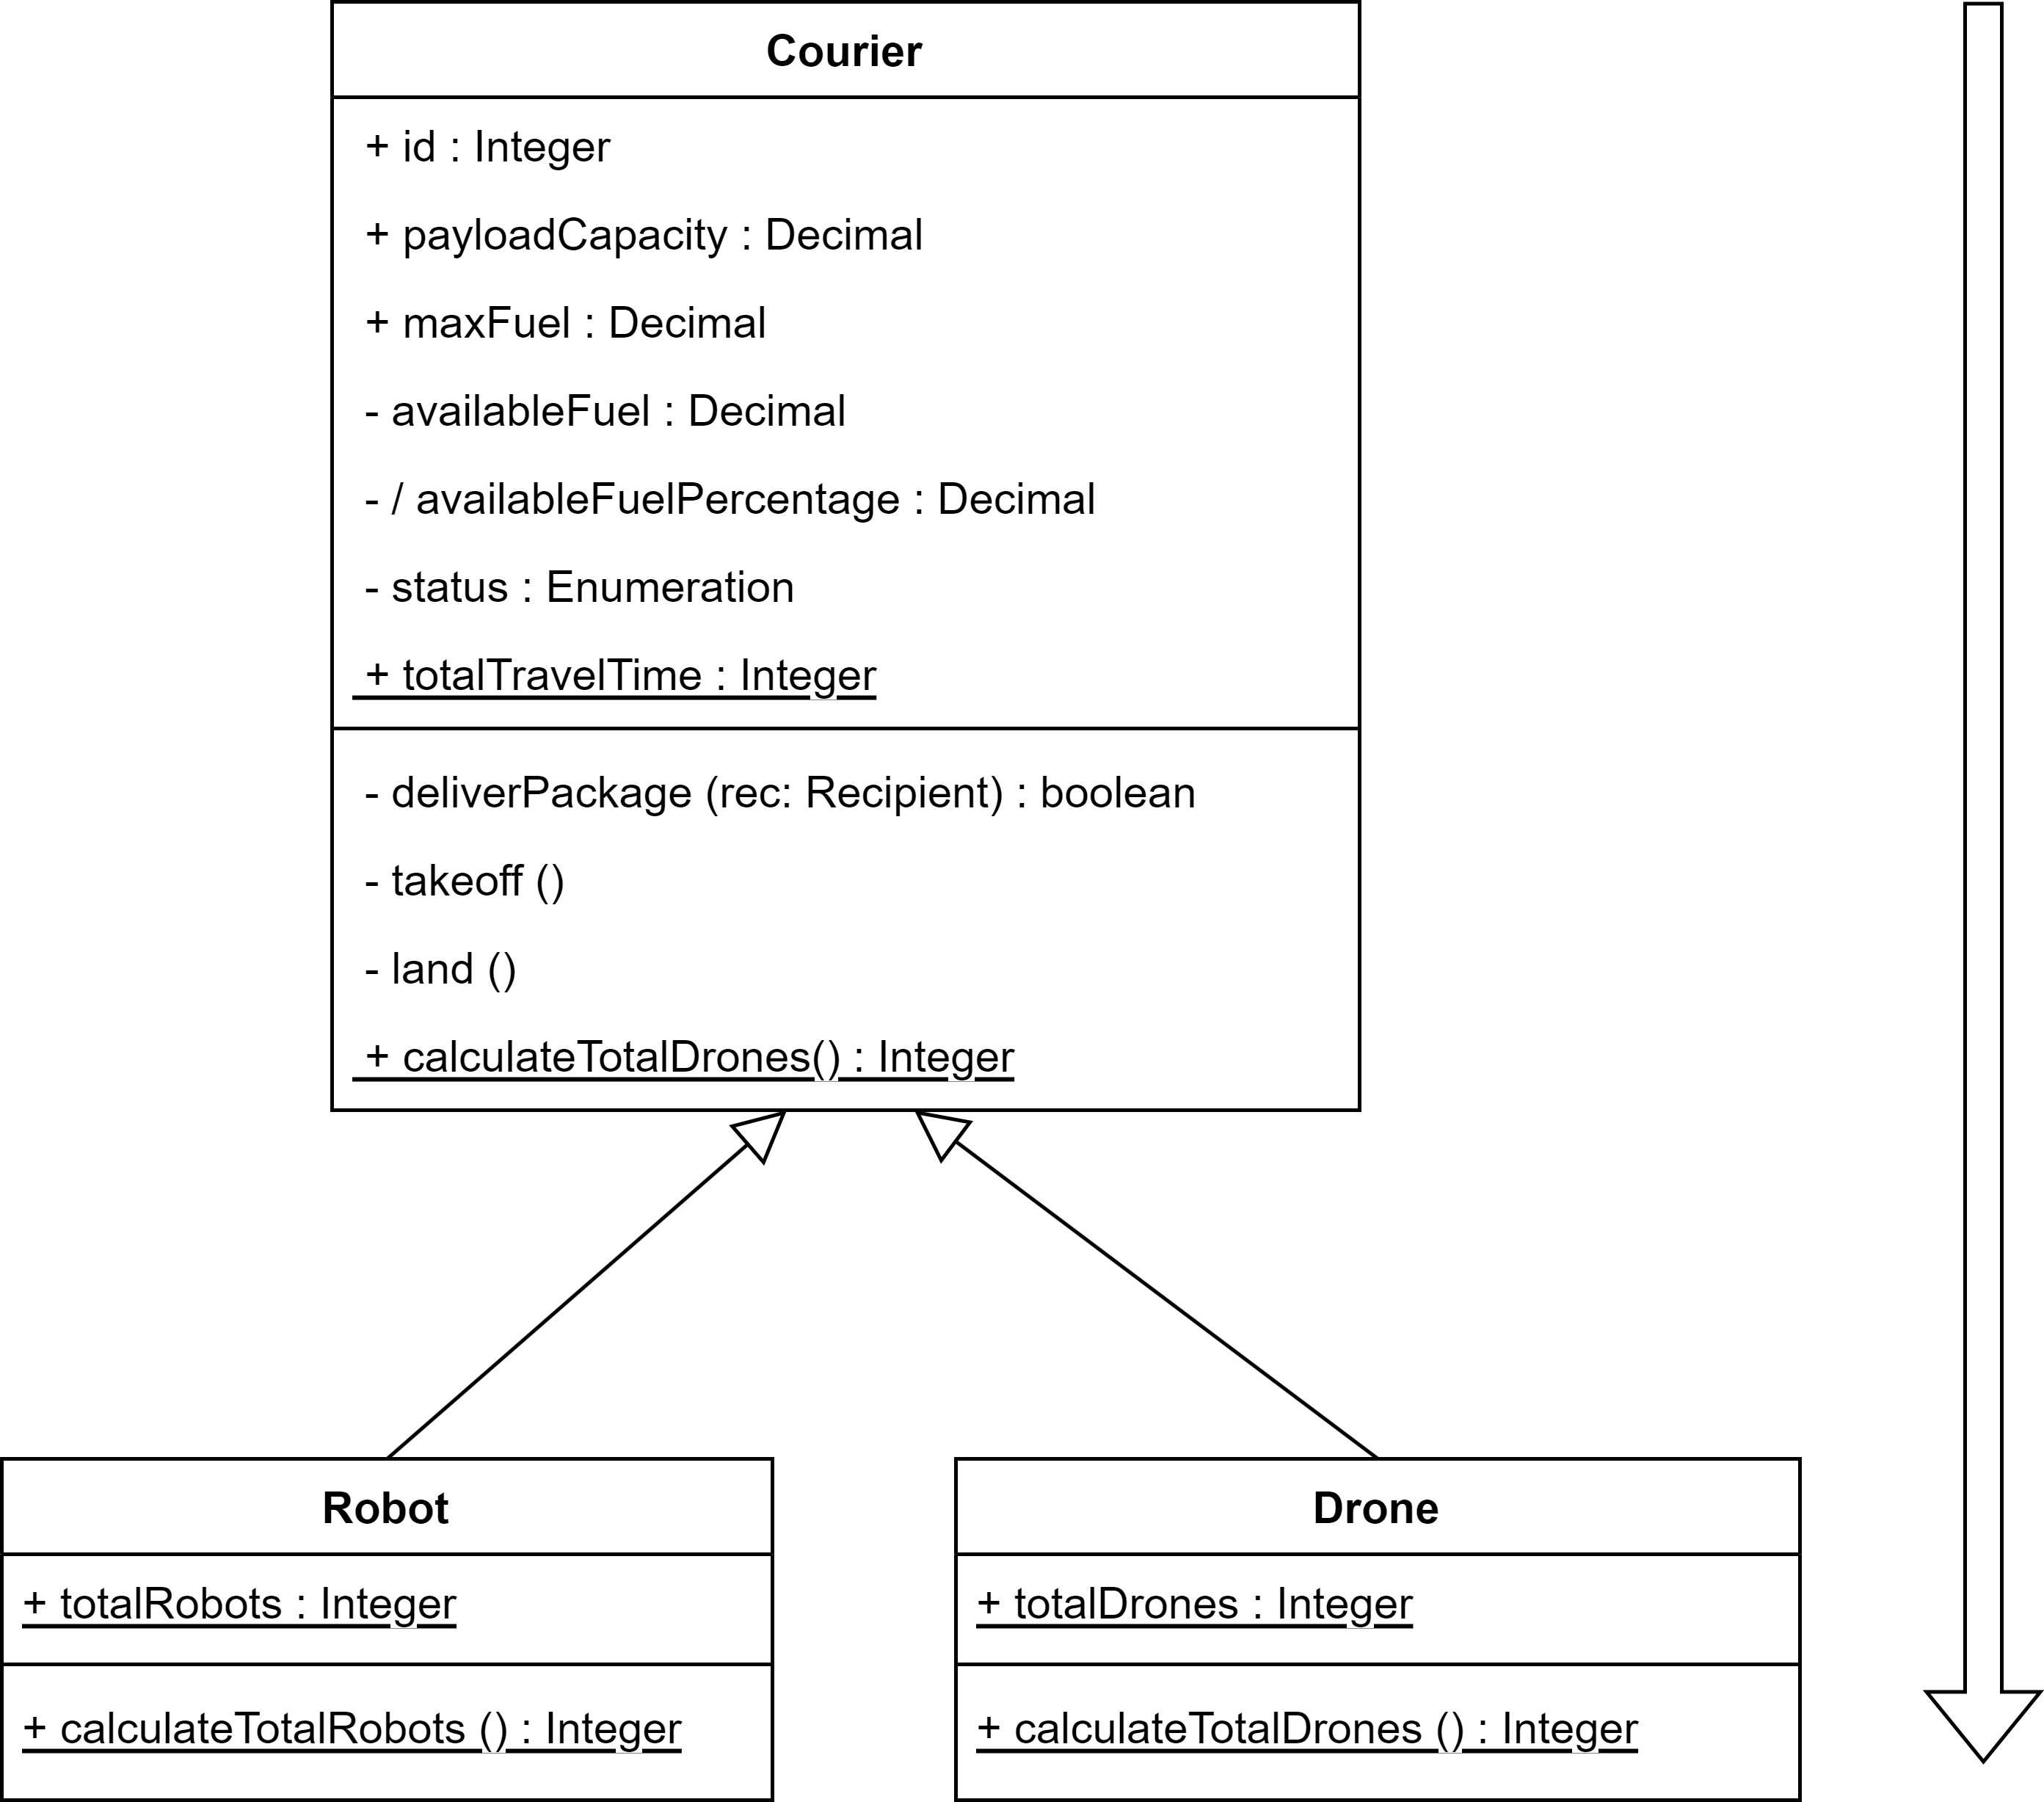
\includegraphics[width=0.7\textwidth]{figures/inheritance/specialization.jpg}
%	\captionof{figure}[Example specialization]{Example of specialization}
%	\label{fig:specialization}
%\end{minipage}





\backmatter
%\listoftodos %remove if no longer needed


% ACHTUNG: ursprüngl: alpha, aber das erzeugt keine Links
%\bibliographystyle{wmaainf}
%\bibliographystyle{alpha}
%\bibliography{refs}
\printbibliography

\clearpage %\cleardoublepage

%-----------------------------------------------------------------------------------------------------------------

%% remove if not needed
%\appendix
%%\pagenumbering{Alph}
%\chapter{Supplemental Information}\label{app:supplemental-information}
%Hier könnte Ihr Anhang stehen!


%-----------------------------------------------------------------------------------------------------------------


\end{document}